% REFERENCIAL TEÓRICO-------------------------------------------------------------------

\chapter{REFERENCIAL TEÓRICO}\label{referencial}


%exemplo de citacao "de nome"
De acordo com \citen{AntonRorres2012}, a definição de um teste de citação com nome do autor pode ser feito segundo este autoexemplo. Outro exemplo de citação, referente a uma declaração completa, é exemplificada no parágrafo a seguir.

Sed feugiat. Cum sociis natoque penatibus et magnis dis parturient montes, nascetur ridiculus mus. Ut pellentesque augue sed urna. Vestibulum diam eros, fringilla et, consectetuer eu, nonummy id, sapien. Nullam at lectus. In sagittis ultrices mauris. Curabitur malesuada erat sit amet massa. Fusce blandit \cite{AtkinsJones2012,AtkinsPaula2014}.


%Inserir seu texto... (remova os comandos \lipsum[*], eles apenas inserem textos "defaul" de exemplo)
%\lipsum[5]


Suspendisse vel felis. Ut lorem lorem, interdum eu, tincidunt sit amet, laoreet vitae, arcu. Aenean faucibus pede eu ante. Praesent enim elit, rutrum at, molestie non, nonummy vel, nisl. Ut lectus eros, malesuada sit amet, fermentum eu, sodales cursus, magna. Donec eu purus. Quisque vehicula, urna sed ultricies auctor, pede lorem egestas dui, et convallis elit erat sed nulla. Donec luctus. Curabitur et nunc. Aliquam dolor odio, commodo pretium, ultricies non, pharetra in, velit. Integer arcu est, nonummy in, fermentum faucibus, egestas vel, odio \cite{AzevedoFernandes2015,BairdCann2011,BaptistaEA2014,BergmanEA2015}.



%------------------ Figura 1
\begin{figure}[H]
\centering
\caption{Título da primeira figura}\label{fig1}
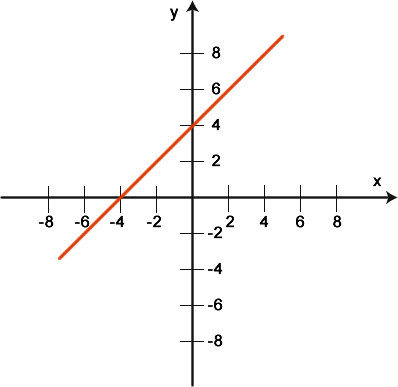
\includegraphics[width=0.5\textwidth]{./dados/figuras/exemplo_fig1.png}
%\fonte{\url{https://ctan.org/lion}}
\fonte{\citen[p. 66]{AntonBusby2006}}
\end{figure}





%Inserir seu texto...
\lipsum[8-9]



\section{Seção secundária}


%Inserir seu texto...
\lipsum[10]

Sed feugiat \citen{BielenkiBarbassa2012}, cum sociis natoque penatibus et magnis dis parturient montes, nascetur ridiculus mus. Ut pellentesque augue sed urna. Vestibulum diam eros, fringilla et, consectetuer eu, nonummy id, sapien. Nullam at lectus. In sagittis ultrices mauris. Curabitur malesuada erat sit amet massa. Fusce blandit. Aliquam erat volutpat. Aliquam euismod. Aenean vel lectus. Nunc imperdiet justo nec dolor \cite{BirdEA2014,Botelho2021,BrandaoEA2012}.


\section{Outra seção secundária}

Vestibulum diam eros, fringilla et, consectetuer eu, nonummy id, sapien \cite{BoyceDiprima2015,CostaAndrade2022}. A Figura~\ref{fig2} ilustra o famoso leão desenhado por Duane Bibby, símbolo do \TeX.


%Inserir seu texto...
\lipsum[12]


%------------------ Figura 2
\begin{figure}[htb]
\centering
%\caption{O famoso leão desenhado por Duane Bibby, símbolo do \TeX}\label{fig1}
\caption{Título da segunda figura}\label{fig2}

\includegraphics[width=0.5\textwidth]{./dados/figuras/tex_lion.png}
\fonte{Disponível em \url{https://ctan.org/lion}}
\end{figure}



%Inserir seu texto...
\lipsum[13-14]



\subsection{Seção terciária}

%Inserir seu texto...
\lipsum[15-17]
